\documentclass[10pt,a4paper]{ctexart}
\usepackage[margin=2cm]{geometry}
\usepackage{graphicx}
\usepackage{hyperref}
\usepackage{amsmath}    % 提供方程环境
\usepackage{physics}    % 简化向量、微分算子语法
\newcommand{\myspace}[1]{\par\vspace{#1\baselineskip}} %自定义空一行
\usepackage{fancyhdr}
\usepackage{wrapfig}
\usepackage{booktabs} % 添加 booktabs 宏包
\usepackage{array}
\usepackage{float}
\usepackage{makecell}
\pagestyle{fancy}
\fancyhf{}  % 清除所有页眉页脚
\fancyfoot[C]{\thepage}  % 在页脚中央设置页码
\renewcommand{\headrulewidth}{0pt}  % 去掉页眉横线
\renewcommand{\footrulewidth}{0pt}  % 去掉页脚横线

\usepackage{hyperref}
\hypersetup{
    colorlinks=true,
    linkcolor=blue,
    filecolor=magenta,      
    urlcolor=cyan,
    pdftitle={Overleaf Example},
    pdfpagemode=FullScreen,
    }

\usepackage{titlesec}

% 重新定义section格式
\titleformat{\section}
  {\normalfont\Large\bfseries}
  {\chinese{section}、}
  {0pt}
  {}

% 给出常用字号的自定义指令
\newcommand{\chuhao}{\fontsize{42pt}{48pt}\selectfont}
\newcommand{\xiaochu}{\fontsize{36pt}{42pt}\selectfont}
\newcommand{\xiaoer}{\fontsize{18pt}{21.6pt}\selectfont}
\newcommand{\sanhao}{\fontsize{16pt}{20pt}\selectfont}
\newcommand{\xiaosan}{\fontsize{15pt}{18pt}\selectfont}
\newcommand{\sihao}{\fontsize{14pt}{18pt}\selectfont}
\newcommand{\xiaosi}{\fontsize{12pt}{16pt}\selectfont}
\newcommand{\wuhao}{\fontsize{10.5pt}{12.6pt}\selectfont}

% 定义中文数字转换
\titleformat{\section}
  {\normalfont\Large\bfseries}
  {\zhnum{section}、}  % 使用\zhnum而不是\chinese
  {0pt}
  {}

% 标题设置
\title{\xiaochu\textbf{物理实验预习报告}}
\author{}
\date{}

\begin{document}

\vspace*{36pt} % 顶部空白

% 居中填写区域
\begin{center}
    
\includegraphics[width = 9cm]{figures/head.png}
    
    \xiaochu\textbf{物理实验预习报告}
    % 预留空白区域
    \vspace{13pt}
    \vspace{13pt}
    \vspace{13pt}
    \vspace{13pt}
    
    \sanhao\textbf{实验名称：\underline{\makebox[10cm]{ 交流电路功率因数实验、组装整流器 }}} \\[10pt]
    \sanhao\textbf{实验桌号：\underline{\makebox[8cm]{ }}} \\[10pt]
    \sanhao\textbf{指导教师：\underline{\makebox[8cm]{ }}} \\[20pt]
    
    % 预留空白区域
    \myspace{7}
    
   \sihao\textbf{班级：\underline{\makebox[6cm]{cc98}}} \\[10pt]
    \sihao\textbf{姓名：\underline{\makebox[6cm]{Hydrofoil}}} \\[10pt]
    \sihao\textbf{学号：\underline{\makebox[6cm]{324010}}} \\[30pt]
    
   \sihao\textbf{实验日期: \underline{\makebox[0.8cm] 2025 }年 \underline{\makebox[0.4cm]12}月\underline{\makebox[0.4cm]18}日  星期\underline{\makebox[0.6cm]四}下午}
    
    \vspace{18pt}
    \sihao 浙江大学物理实验教学中心
    
\end{center}

\newpage

    \section{实验综述}
    
    \xiaosi （自述实验现象、实验原理和实验方法，不超过500字，5分）
    
    \myspace{0}
    
    \subsubsection*{日光灯电路与功率因数的提高：}

    日光灯是一种典型的电感性负载电路，它主要由灯管$L$、镇流器$M$、启辉器$S$组成，如图所示。

    \begin{figure}[H]
    \centering
    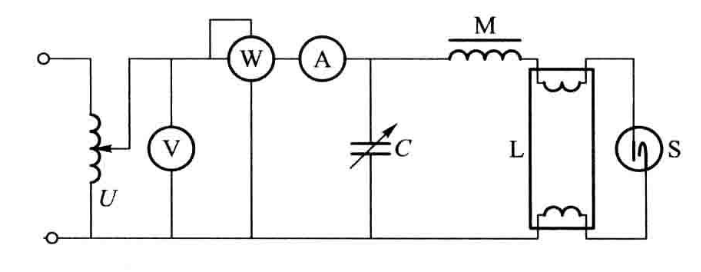
\includegraphics[width=10cm]{figures/日光灯.png}
    \caption{日光灯电路工作原理图}
    \label{fig:图1}
    \end{figure}  

    日光灯通电后，启辉器辉光放电接通电路，电流加热灯丝使其发射电子并气化管内液汞。随后启辉器自动断开，导致串联的镇流器产生瞬间高压，击穿灯管内的汞蒸气形成弧光放电。放电时高速电子撞击汞原子辐射出紫外线，紫外线激发管壁荧光粉吸收能量并发出可见光。灯管点亮后，镇流器利用感抗限制电流，维持其稳定发光。
    
    交流电路中的负载分为阻性负载、容性负载、感性负载。阻性负载电流和电压相位相同，容性负载电流超前电压$90^{\circ}$，感性负载电流落后电压$90^{\circ}$。
    
    如果用 $I_L$ 作为相位的参考方向，下图是它们之间的相位矢量图，由图可见 $I_L$ 与 $U_R$ 同相。而纯电感 $L $上的电压 $U_L$ 比 $I_L$ 超前 $\pi/2$，合成的 $U $是总电压的幅值，$\varphi $是 $I_L$ 落后$U$ 的相位角。
    
    \begin{figure}[H]
    \centering
    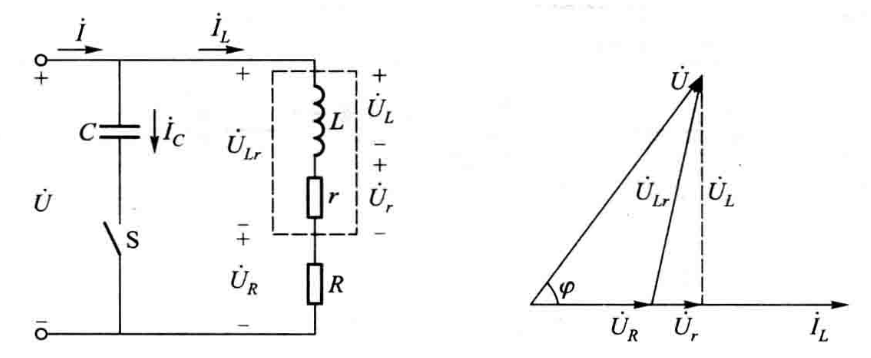
\includegraphics[width=10cm]{figures/相位.png}
    \caption{相位关系}
    \label{fig:图2}
    \end{figure}

    \
    

    \begin{wrapfigure}{r}{0.4\textwidth}
    \centering
    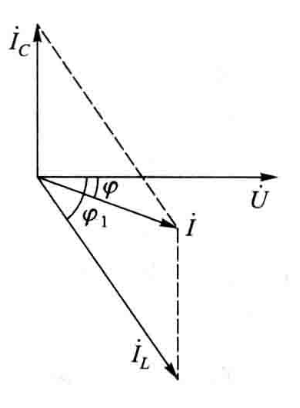
\includegraphics[width=3cm]{figures/并联.png}
    \caption{功率因数的放大}
    \label{fig:图1}
    \end{wrapfigure}

    \

对应提高电感性电路的功率因数，常用的方法就是在靠近感性负载端并联电容器，其电路图如左图所示，由相量图可知原感性负载电流滞后于电压$ \varphi $当并联电容以后
，只要电容的大小选择得当，就可以使并联电容以后的总电流小于原来电感中的电流，使$ \varphi' < \varphi $使功率因数得到提高。  

    \subsubsection*{各种电压的定义及波形因素}
    
    峰峰电压\(V_{PP}\)：表示正弦波峰到波峰之间的电压幅度；
    
    峰值电压\(V_{P}\)：表示正向脉动电压从零电平到最高电压之间的幅度；
    
    平均值电压：\(\bar{V}=\frac{1}{T} \int_{0}^{T} u(t) dt\)；
    
    有效值电压：\(\dot{V}=\sqrt{\frac{1}{T} \int_{0}^{T} u^{2}(t) dt}\)。
    
    \subsubsection*{各波形间的相互关系}
    
    波形系数：\(K_{F}=\frac{\dot{V}}{\bar{V}}\)；波峰系数：\(K_{P}=\frac{V_{P}}{\dot{V}}\)；
    
    由上述两式可得：\(\bar{V}=\frac{V_{P}}{K_{F} \cdot K_{P}}\)。
    
    \begin{wrapfigure}{r}{0.4\textwidth}
    \centering
    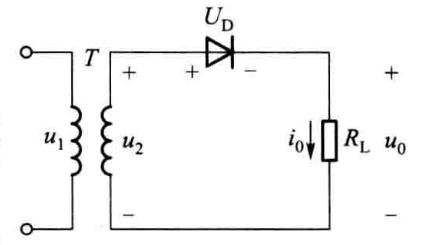
\includegraphics[width=6cm]{figures/半波.png}
    \caption{半波整流电路}
    \label{fig:图1}
    \end{wrapfigure}
    
    
    \subsubsection*{整流电路的类型及特点}

    
    \textbf{1.半波整流}
    
    二极管的反向耐压：电阻负载时承受的反向最大电压为\(\sqrt{2}V_{2}\)；电容负载时承受的反向最大电压为\(2\sqrt{2}V_{2}\)。
    
    输入输出电压关系：输入\(u=\sqrt{2}V_{2}\sin\omega t\)，在二极管导通时忽略电路损耗与门限电压，则：
    
    \(\overline{V_{0}}=\frac{1}{2\pi} \int_{0}^{\pi} u_{2} d(\omega t)=\frac{\sqrt{2}}{\pi}V_{2}≈0.45V_{2}\)。
    
    \begin{wrapfigure}{r}{0.4\textwidth}
    \centering
    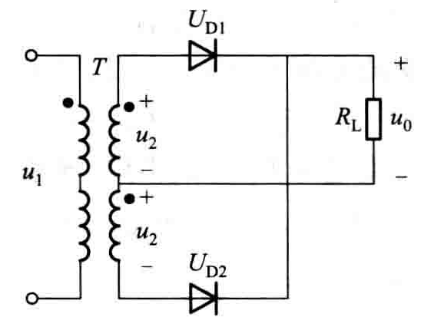
\includegraphics[width=5cm]{figures/全波.png}
    \caption{全波整流电路}
    \label{fig:图1}
    \end{wrapfigure}
    
    \textbf{2.全波整流}
    
    滤波效果及二极管承受反向最大压降与半波整流相同。
    
    优点：利用了电源的正、负周期，电源脉动大大减小。缺点：需要两个整流二极管，变压器需中心抽头，结构相对复杂。
    
    \textbf{3.桥式整流}
    
    滤波效果与前两者相同。二极管承受的最大反向压降由两只二极管共同分担。

    \begin{figure}[H]
    \centering
    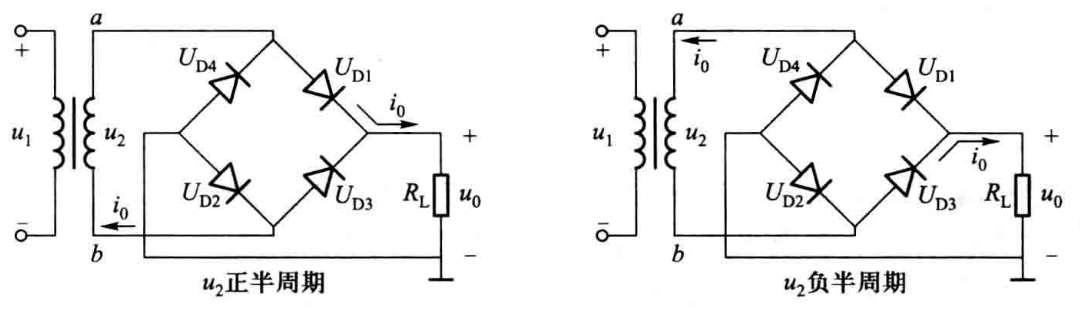
\includegraphics[width=10cm]{figures/桥式.png}
    \caption{桥式整流电路}
    \label{fig:图2}
    \end{figure}

    
    \subsubsection*{滤波电路}
    
    滤波原理（以 RC 为例）：当u为正半周期时，二极管导通，对电容充电，因二极管导通时内阻很小，电容很快被充到峰值。当负半周期时，二极管截止，电容放电，时间常数\(\tau = RC\)。当\(\tau \gg T\)时，电容上电压刚释放一小部分，下一周期二极管又导通，电容充电，如此即可保持输出电压稳定。



    \section{实验重点}
    
    \xiaosi（简述本实验的学习重点，不超过100字，3分）

    \begin{enumerate}
        \item 理解功率因数的物理意义；
        \item 掌握提高感性电路功率因数的方法；
        \item 主席日光灯的工作原理，掌握测量日光灯功率的方法；
        \item 根据实验室提供的元件，完成各种整流电路的设计；
        \item 熟悉电子示波器的使用，了解一些常用电子元件的使用方法；
        \item 了解整流器作用，以及整流电路和滤波电路的功能。
    \end{enumerate}
    
    \section{实验难点}
    
    \xiaosi（简述本实验的实现难点，不超过100字，2分）

    \begin{enumerate}
        \item 电路搭建精度要求高：半波、全波、桥式整流电路的接线逻辑不同（如全波需变压器中心抽头、桥式需四只二极管合理排布），且元件（二极管、电容、电阻）极性和连接位置易出错，影响电路导通与整流效果。
        \item 仪器操作与波形观测难度：需熟练掌握示波器的连接方式、参数调节（如峰峰值、有效值测量），且滤波前后波形变化细微，需精准区分并记录，读数存在天然浮动误差。
        \item 反向耐压与电路安全控制：二极管反向耐压值需匹配电路电压（如半波整流电容负载时反向电压达\(2\sqrt{2}V_{2}\)），且变压器禁止短路，操作中需规避过载、接线错误等安全风险。
        \item 误差控制与数据分析：实际元件非理想特性（如二极管反向漏电流、元件内阻）、输入电压波动等因素易导致实验数据与理论值偏差，需准确识别误差来源并合理分析。
    \end{enumerate}

\newpage


\sihao\textbf{注意事项：}
\xiaosi
\begin{enumerate}
    \item  用 PDF 格式上传“实验报告”，文件名：学生姓名+学号+实验名称+周次。
    \item  “实验报告”必须递交在“学在浙大”的本课程的对应实验项目的“作业”模块内。
    \item  “实验报告”成绩必须在“浙江大学物理实验教学中心网站”-“选课系统”内查询。
    \item 教学评价必须在“浙江大学物理实验教学中心网站”-“选课系统”内进行，学生必须进行教学评价，才能看到实验报告成绩，教学评价必须在本次实验结束后 3 天内进行。
\end{enumerate}

\vspace{1cm}
\xiaosi\centering \textbf{浙江大学物理实验教学中心制}

\end{document}